\documentclass[11pt, a4paper]{article}
\usepackage[utf8]{inputenc}
\usepackage[slovene]{babel}
\usepackage{amsmath}
\usepackage{amsfonts}
\usepackage{graphicx}
\usepackage{booktabs}

\title{Domača naloga 2: Gauss-Legendrove kvadrature}
\author{Anže Judež}
\date{\today}

\begin{document}

\maketitle

\section{Splošen Opis naloge}
Cilj naloge je bila izpeljava in implementacija sestavljenega Gauss-Legendrovega integracijskega pravila na dveh točkah. Metodo smo uporabili za izračun integrala funkcije:
\begin{equation}
    I = \int_{0}^{5} \frac{\sin x}{x} dx
\end{equation}
na 10 decimalk natančno. Pri tem smo morali oceniti število potrebnih izračunov funkcijskih vrednosti in analizirati napako metode.

\section{Izpeljava metode in napake}
Osnovno Gauss-Legendrovo pravilo na dveh točkah za interval $[-1, 1]$ je podano z:
\begin{equation}
    \int_{-1}^{1} f(\xi) d\xi \approx f\left(-\frac{1}{\sqrt{3}}\right) + f\left(\frac{1}{\sqrt{3}}\right)
\end{equation}
Za splošni interval $[x_i, x_{i+1}]$ dolžine $h$ pravilo prevedemo z uvedbo nove spremenljivke, kar nam da:
\begin{equation}
    \int_{x_i}^{x_{i+1}} f(x) dx \approx \frac{h}{2} \left[ f(x_{i,1}) + f(x_{i,2}) \right]
\end{equation}
kjer sta $x_{i,1}$ in $x_{i,2}$ vozlišči, preslikani na podinterval.

\subsection{Ocena napake}
Teoretična napaka $R_f$ za osnovno Gauss-Legendrovo pravilo na dveh točkah za interval $[-1, 1]$ je podana z izrazom:
\begin{equation}
    R_f = \frac{f^{(4)}(\eta)}{135}, \quad \eta \in (-1, 1).
\end{equation}
Ocena je povzeta po literaturi \cite{orel2004} (str. 132). Formulo izpeljemo s pomočjo Hermiteovega interpolacijskega polinoma, kjer izkoristimo lastnost, da je Gauss-Legendrovo pravilo z $n$ točkami eksaktno za vse polinome stopnje $2n-1$ ali manj. V našem primeru ($n=2$) je pravilo eksaktno za polinome stopnje 3, zato je vodilni člen napake povezan s četrtim odvodom funkcije $f$.

Pri sestavljenem pravilu z $n$ podintervali dolžine $h = \frac{b-a}{n}$ se napaka na celotnem intervalu $[a, b]$ poenostavi v:
\begin{equation}
    R_{f, \text{sest}} = -\frac{(b-a)h^4}{4320} f^{(4)}(\eta).
\end{equation}

\section{Implementacija in rezultati}
Naloga je implementirana v jeziku Julia v obliki paketa \texttt{Naloga02}. Za določanje števila korakov smo uporabili metodo podvajanja števila intervalov (Double-Step method). Napako smo ocenili s pomočjo Rungejevega pravila:
\begin{equation}
    \epsilon \approx \frac{|I_{2n} - I_n|}{2^p - 1} = \frac{|I_{2n} - I_n|}{15}
\end{equation}

\begin{figure}[h]
    \centering
    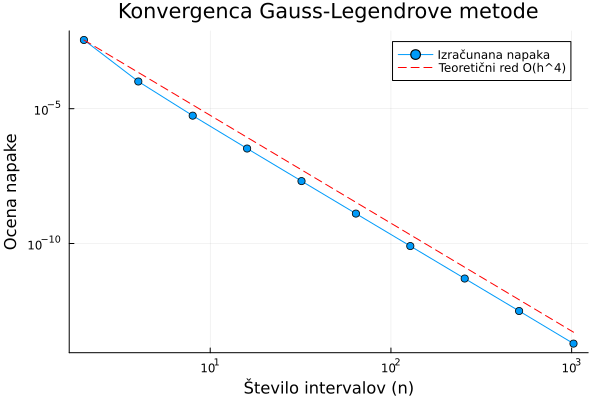
\includegraphics[width=0.7\textwidth]{konvergenca_gauss.png}
    \caption{Graf padanja napake v odvisnosti od števila intervalov.}
\end{figure}

\subsection{Numerični izračun}
Pri računanju integrala funkcije $\frac{\sin x}{x}$ na intervalu $[0, 5]$ smo dobili naslednje rezultate:

\begin{table}[h]
    \centering
    \begin{tabular}{ccc}
        \toprule
        Število intervalov ($n$) & Približek integrala & Ocena napake \\
        \midrule
        1   & 1.604526529428197 & --- \\
        4   & 1.550019196137019 & $1.02 \cdot 10^{-4}$ \\
        16  & 1.549931574721094 & $3.33 \cdot 10^{-7}$ \\
        64  & 1.549931246229614 & $1.29 \cdot 10^{-9}$ \\
        128 & 1.549931245024972 & $8.03 \cdot 10^{-11}$ \\
        \bottomrule
    \end{tabular}
    \caption{Konvergenca integrala funkcije $\text{sinc}(x)$ na intervalu $[0, 5]$.}
\end{table}

Za dosego natančnosti $10^{-10}$ smo potrebovali 128 podintervalov. Ker na vsakem podintervalu izračunamo dve funkcijski vrednosti, je skupno število izračunov funkcijske vrednosti enako 256.

\section{Zaključek}
Sestavljeno Gauss-Legendrovo pravilo se je izkazalo za zelo robustno. Kljub majhnemu številu točk smo hitro dosegli visoko natančnost, kar potrjuje teoretična pričakovanja o metodi reda $O(h^4)$. Koda je preverjena z enotskimi testi na polinomih stopnje 3, kjer metoda vrne eksaktne rezultate.

\begin{thebibliography}{9}

\bibitem{textbook} 
M. Vuk, \textit{Navodila za pripravo domačih nalog in opisi nalog (poglavja 17 in 18)}, Učbenik za numerične metode, 2026.

\bibitem{orel2004}
B. Orel, \textit{Osnove numerične matematike}, Fakulteta za računalništvo in informatiko, 2004.

\bibitem{plestenjak2015}
B. Plestenjak, \textit{Razširjen uvod v numerične metode}, DMFA - založništvo, 2015.

\end{thebibliography}

\end{document}